\section*{Chapitre 3- Activité 1 : Retour sur la symétrie axiale}

Tracer les symétries par rapport aux droite $(d)$.

\begin{minipage}[t]{0.45\textwidth}
    
    \begin{figure}[H]
        \centering
        \begin{tikzpicture}
            \def\mypath{(-3,2) -- (-1,2) --(-2,0) -- (1,3)--(0,1)--(-2,2)}
            \draw [thick]\mypath ;
            \draw (-2,-2)--(3,3) node [right]{$(d)$} ;
            % \draw [cm={0,1,1,0,(0,0)},dashed] \mypath;%Matrice de transformation inverse X et Y
            \draw [dotted](-3,-3) grid (4,4);
        \end{tikzpicture}
    \end{figure}
\end{minipage}
\hfill
\begin{minipage}[t]{0.45\textwidth}
    
    \begin{figure}[H]
        \centering
        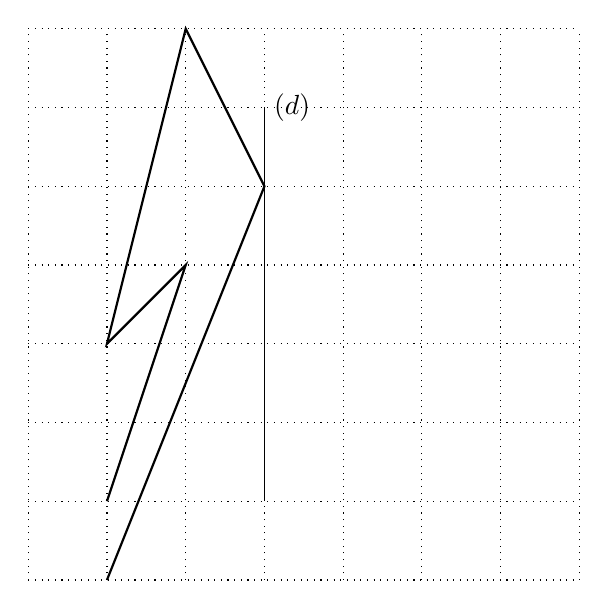
\begin{tikzpicture}
            \def\mypath{(-2,-2) -- (-1,1) --(-2,0) -- (-1,4)--(0,2)--(-2,-3)}
            \draw [thick]\mypath ;
            \draw (0,-2)--(0,3) node [right]{$(d)$} ;
            % \draw [cm={-1,0,0,1,(0,0)},dashed] \mypath;%Matrice de transformation inverse X et Y
            \draw [dotted](-3,-3) grid (4,4);
        \end{tikzpicture}
    \end{figure}
\end{minipage}

\begin{minipage}[t]{0.45\textwidth}
    
    \begin{figure}[H]
        \centering
        \begin{tikzpicture}
            \def\mypath{(-2,-2) -- (0,-1) --(3,-2) -- (2,-1)--(-1,-3)--(-2,-1)}
            \draw [thick]\mypath ;
            \draw (-2,0)--(3,0) node [right]{$(d)$} ;
            % \draw [cm={1,0,0,-1,(0,0)},dashed] \mypath;%Matrice de transformation inverse X et Y
            \draw [dotted](-3,-3) grid (4,4);
        \end{tikzpicture}
    \end{figure}
\end{minipage}
\hfill
\begin{minipage}[t]{0.45\textwidth}
    
    \begin{figure}[H]
        \centering
        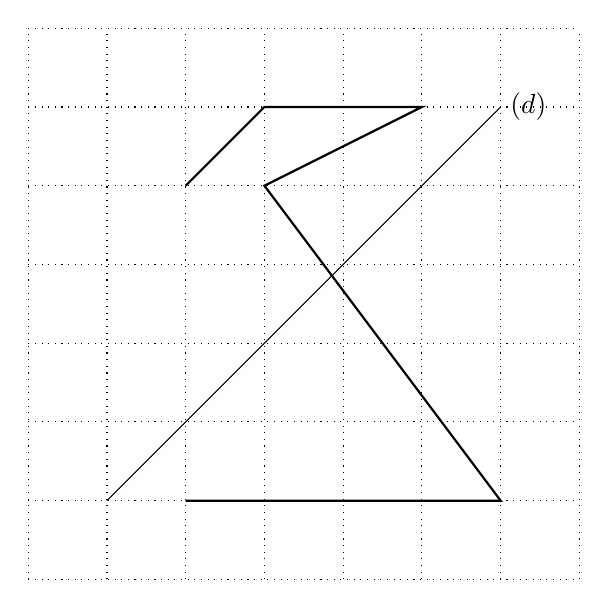
\begin{tikzpicture}
            \def\mypath{(-1,-2) -- (3,-2) --(0,2) -- (2,3)--(0,3)--(-1,2)}
            \draw [thick]\mypath ;
            \draw (-2,-2)--(3,3) node [right]{$(d)$} ;
            % \draw [cm={0,1,1,0,(0,0)},dashed] \mypath;%Matrice de transformation inverse X et Y
            \draw [dotted](-3,-3) grid (4,4);
        \end{tikzpicture}
    \end{figure}
\end{minipage}

\begin{minipage}[t]{0.45\textwidth}
    
    \begin{figure}[H]
        \centering
        \begin{tikzpicture}
            \def\mypath{(-2,-1) -- (2,-1) --(3,-2) -- (0,-1)--(-1,-3)--(-2,-1)}
            \draw [white](-3,-3) grid (4,4);
            \draw [thick]\mypath ;
            \draw (-2,0)--(3,0) node [right]{$(d)$} ;
            % \draw [cm={1,0,0,-1,(0,0)},dashed] \mypath;%Matrice de transformation inverse X et Y
        \end{tikzpicture}
    \end{figure}
\end{minipage}
\hfill
\begin{minipage}[t]{0.45\textwidth}
    
    \begin{figure}[H]
        \centering
        \begin{tikzpicture}
            \def\mypath{(-1,-2) -- (3,-2) --(2,2)--(-1,-2)--(3,1)}
            \draw [white](-3,-3) grid (4,4);
            \draw [thick]\mypath ;
            \draw (-2,-2)--(3,3) node [right]{$(d)$} ;
            % \draw [cm={0,1,1,0,(0,0)},dashed] \mypath;%Matrice de transformation inverse X et Y
        \end{tikzpicture}
    \end{figure}
\end{minipage}